\documentclass{article}
\usepackage{enumitem} % For customized lists
% Add more packages here that you need!
\usepackage{graphicx} 
\usepackage[margin=1in]{geometry} 
\usepackage{amsmath,amsthm,amssymb}
\usepackage[noend]{algpseudocode}
\usepackage{algorithm}
% \usepackage{algpseudocode}
\usepackage{amsfonts}
\usepackage{amsmath}
\usepackage{float}
\usepackage{mathrsfs}
\usepackage{booktabs}
\usepackage{caption}
\captionsetup{justification=centering}
\captionsetup{skip=5pt}
\usepackage[nodisplayskipstretch]{setspace}
\setstretch{1}
\setlength{\abovedisplayskip}{0em}
\setlength{\belowdisplayskip}{0.5em}
\makeatletter
\def\BState{\State\hskip-\ALG@thistlm}
\makeatother

\hyphenation{op-tical net-works semi-conduc-tor}

\begin{document}

\title{Assembly Instructions for Forklift Device}
\author{}
\date{}

\maketitle

\section{Introduction}
These instructions will guide you through the steps needed to assemble a forklift device from the provided components.

\section{Tools Required}
\begin{itemize}
    \item Small Phillips screwdriver
    \item Soldering station
\end{itemize}

\section{Parts Required}
\begin{itemize}
    \item fork * 1
    \item gear box * 2
    \item rack * 2
    \item gear * 2
    \item motor * 2

    \begin{figure}[H]
        \centering
        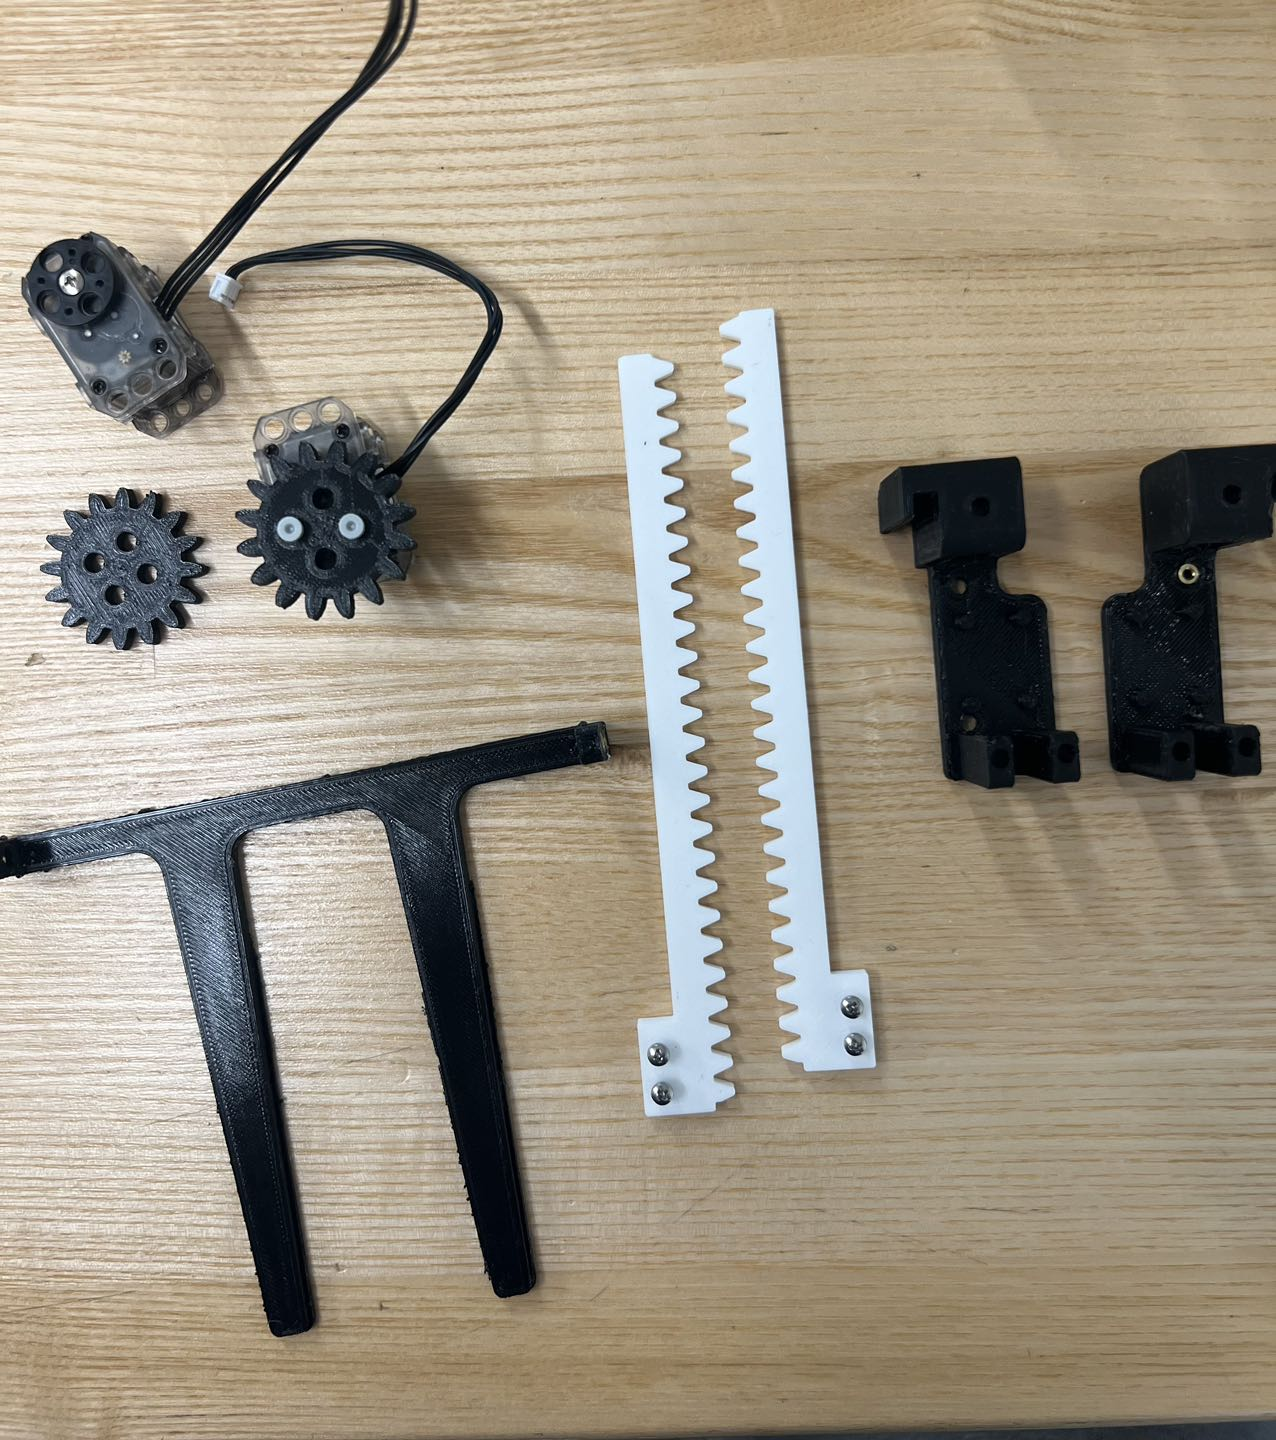
\includegraphics[width=0.45\textwidth]{2.jpg}
        \captionsetup{justification=centering}
        \caption{}
    \end{figure}    

\end{itemize}

\section{Assembly Steps}
Follow these steps to assemble your forklift device:\\


\begin{enumerate}[label=Step \arabic*:,leftmargin=*,align=left]
    \item \textbf{Prepare the Case:}
    Weld two 2.5mm screw nuts onto each gear box and two 2.5mm screw nuts onto each side of fork.
    \begin{figure}[H]
        \centering
        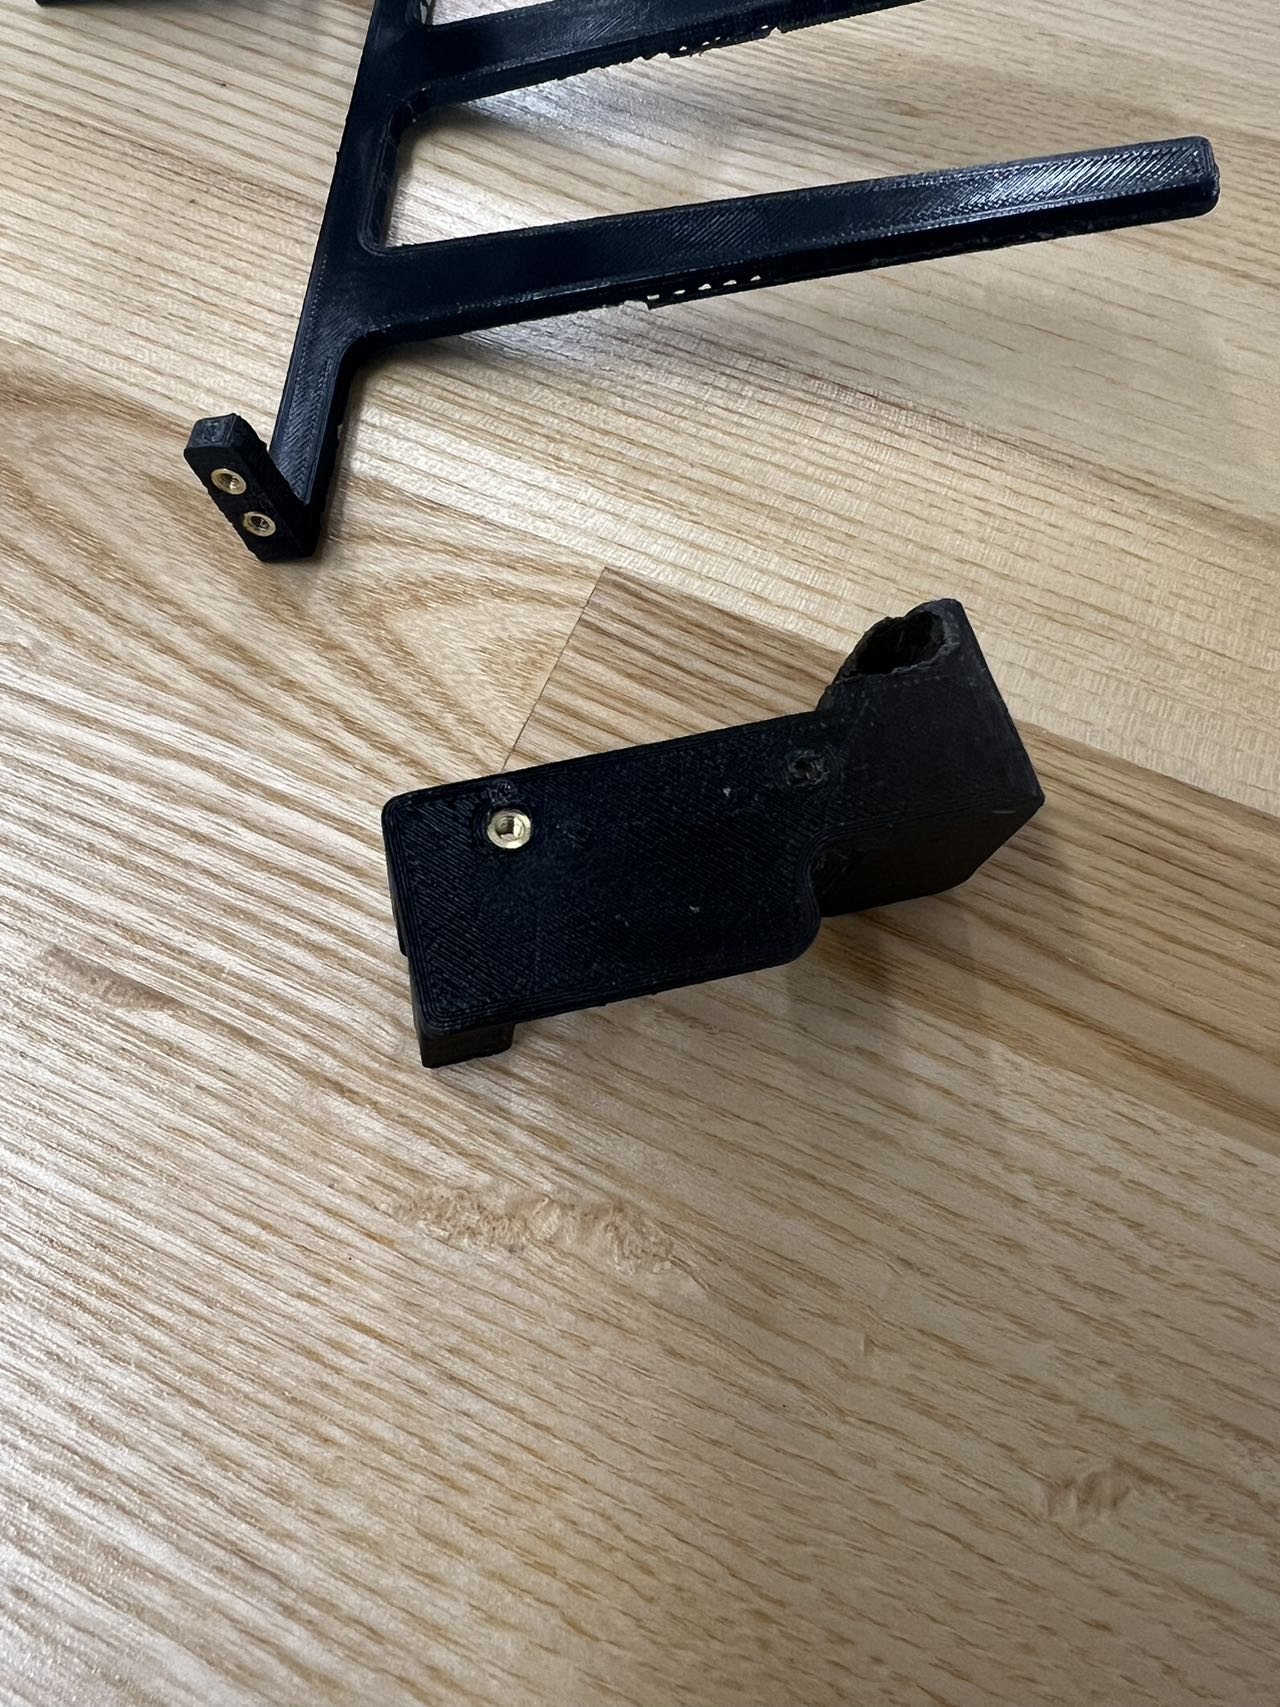
\includegraphics[width=0.37\textwidth]{1.jpg}
        \captionsetup{justification=centering}
        \caption{}
    \end{figure}  

    \item \textbf{Link fork:}
    Link each side of fork with rack by two 2.5mm screws.

    \begin{figure}[H]
        \centering
        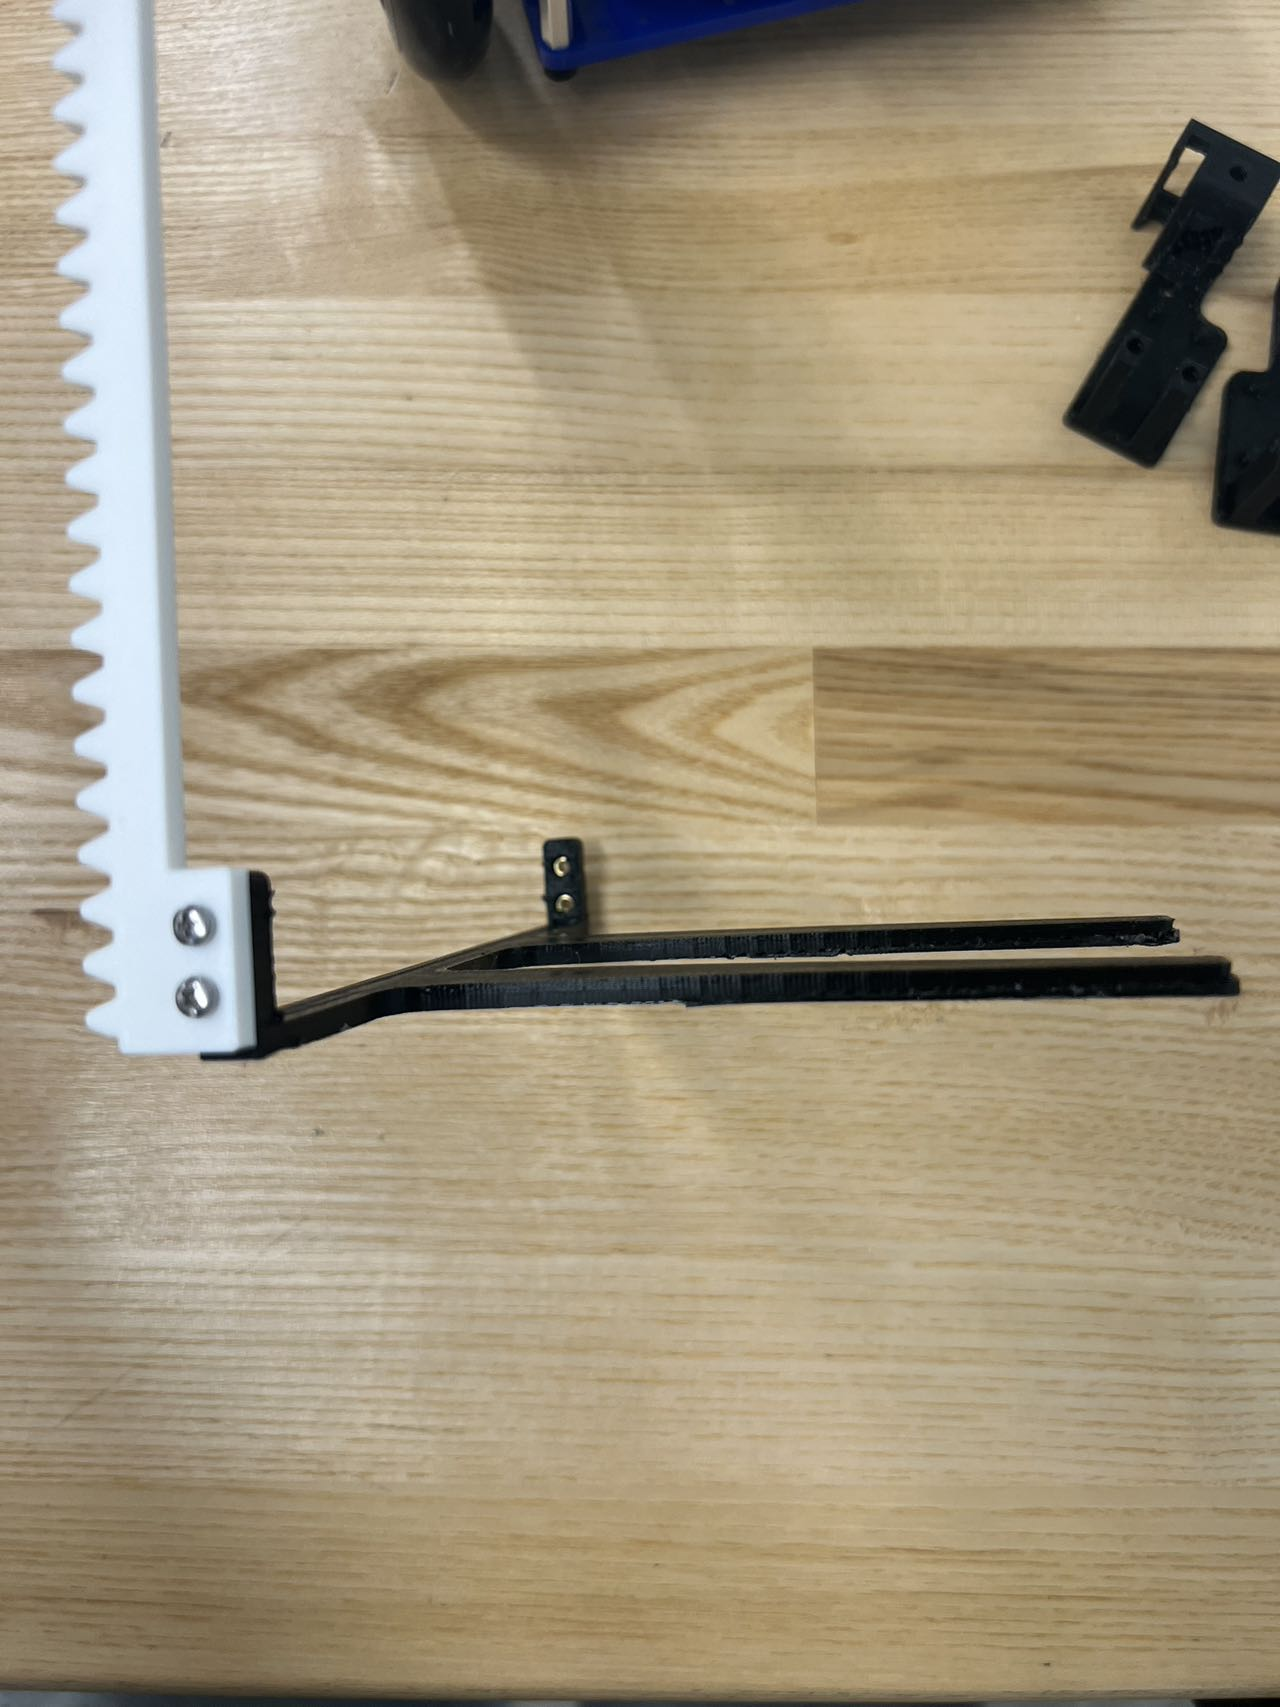
\includegraphics[width=0.40\textwidth]{3.jpg}
        \captionsetup{justification=centering}
        \caption{}
    \end{figure}  

    \item \textbf{Link gear:}
    Link each motor output shaft with gear by two 2.5mm pins.

    \begin{figure}[h]
        \centering
        \begin{minipage}{0.36\textwidth}
            \centering
            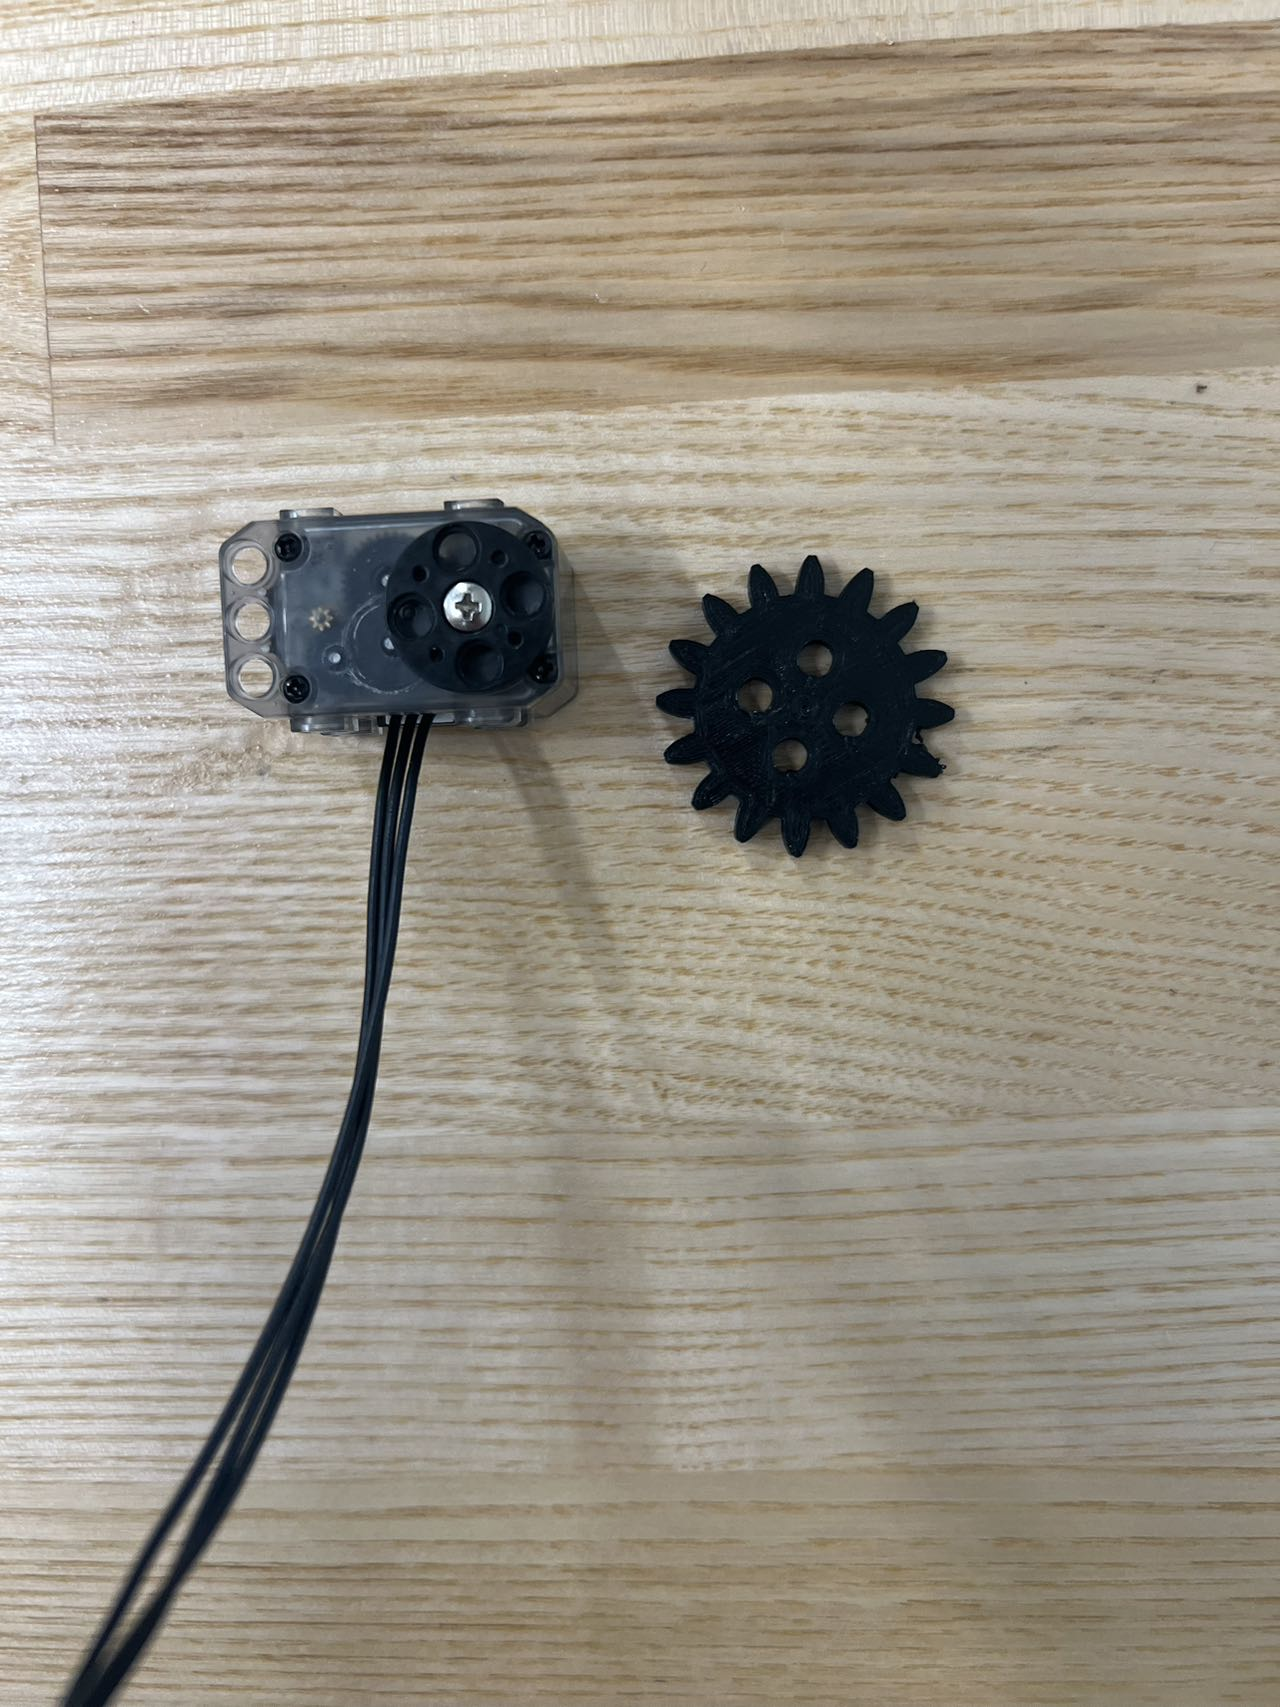
\includegraphics[width=\linewidth]{4.jpg} 
            \caption{}
        \end{minipage}
        \hspace{10pt}
        \begin{minipage}{0.36\textwidth}
            \centering
            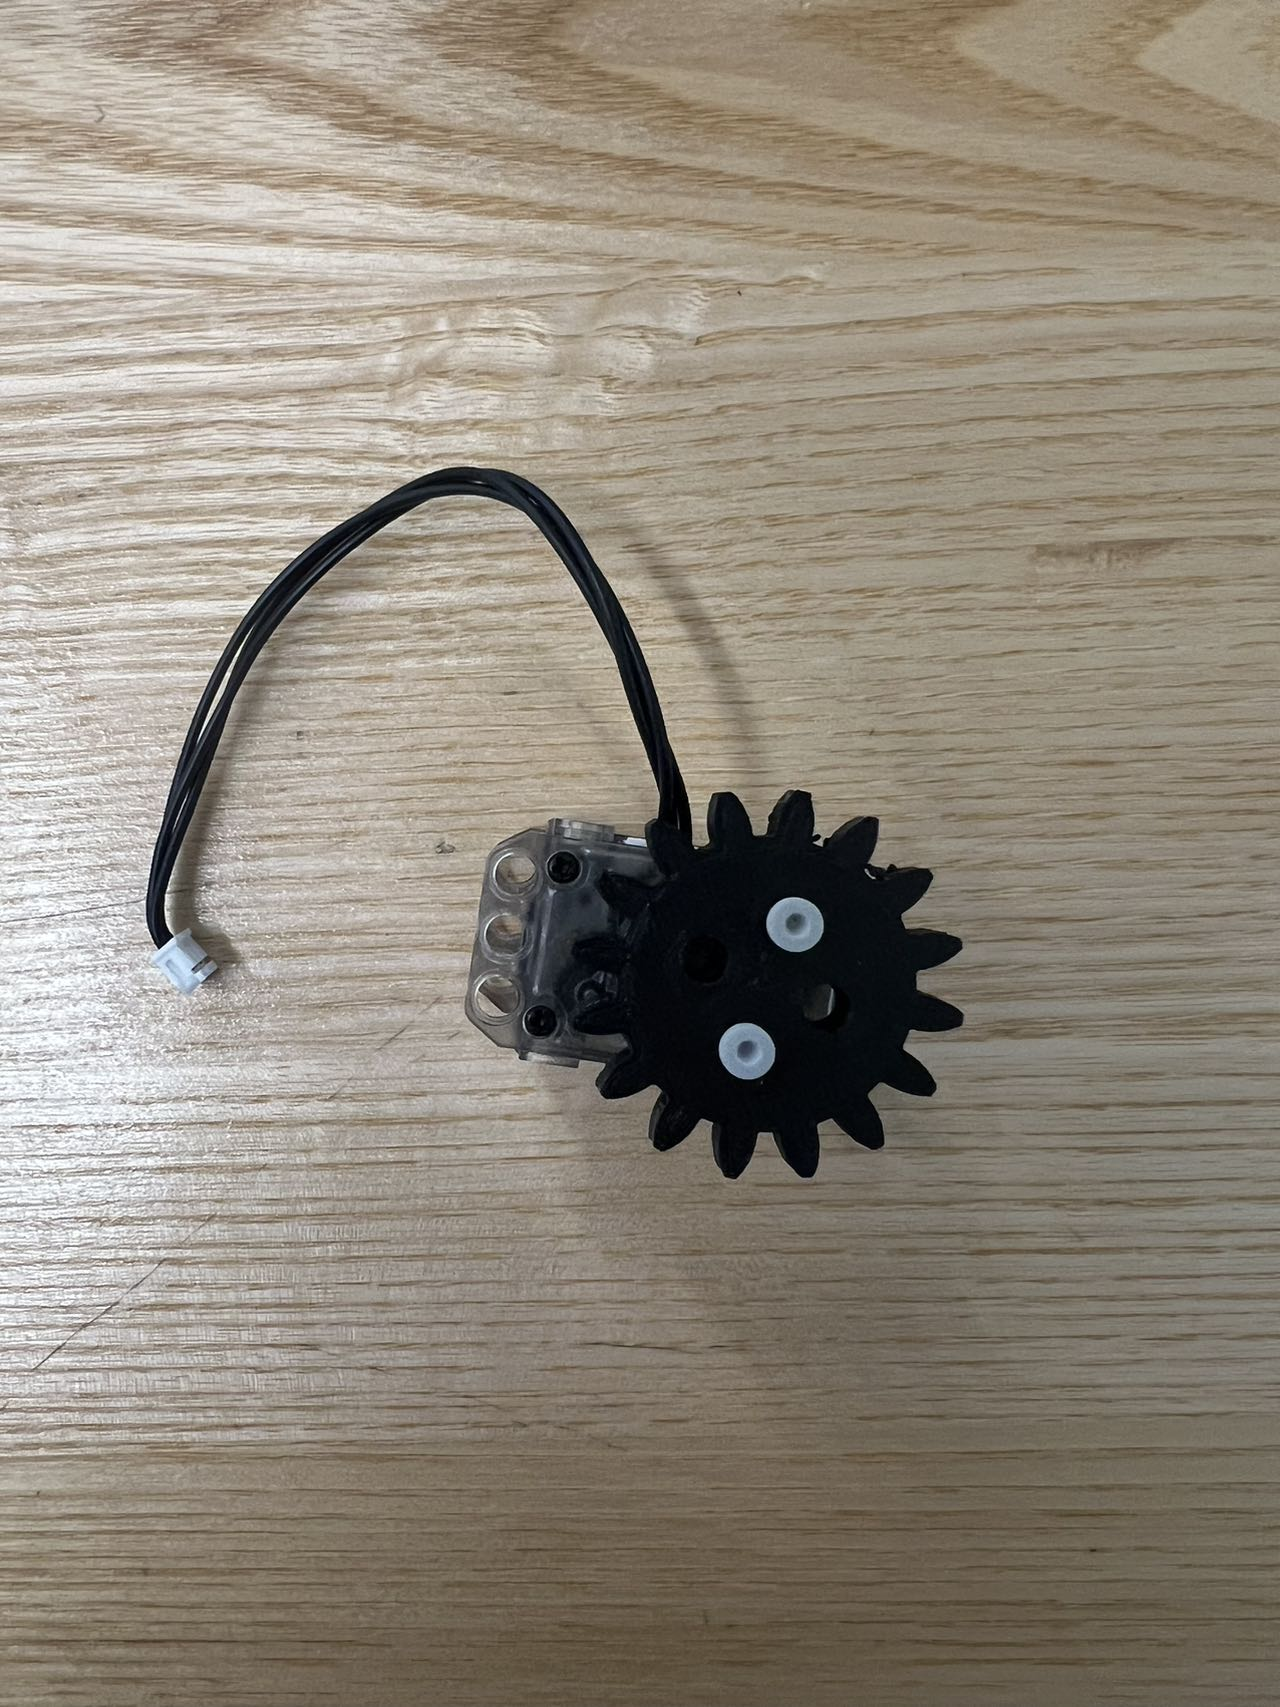
\includegraphics[width=\linewidth]{5.jpg} 
            \caption{}
        \end{minipage}
    \end{figure}

    \item \textbf{Link gear and rack:}
    Set up the each motor into the gear box and link each gear with rack.

    \begin{figure}[h]
        \centering
        \begin{minipage}{0.358\textwidth}
            \centering
            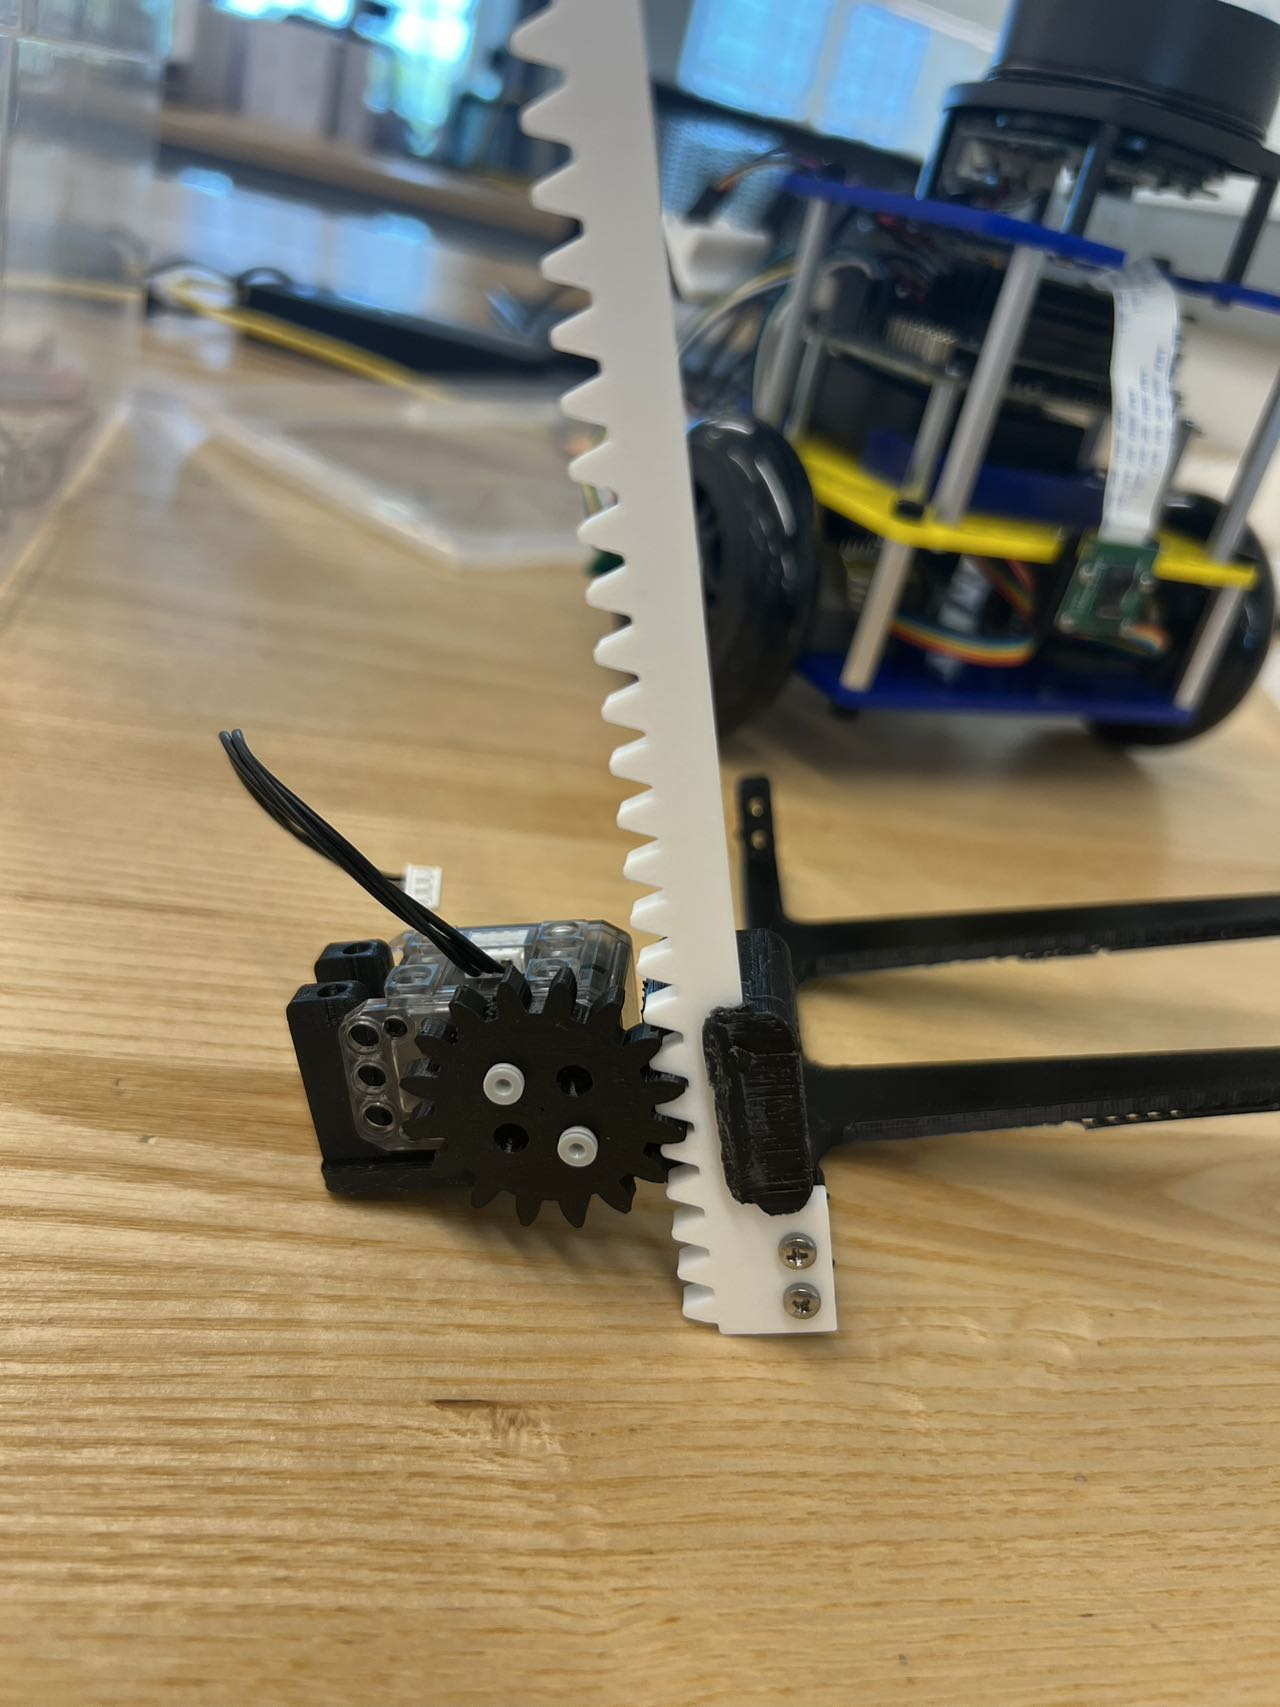
\includegraphics[width=\linewidth]{6.jpg} 
            \caption{}
        \end{minipage}
        \hspace{10pt}
        \begin{minipage}{0.358\textwidth}
            \centering
            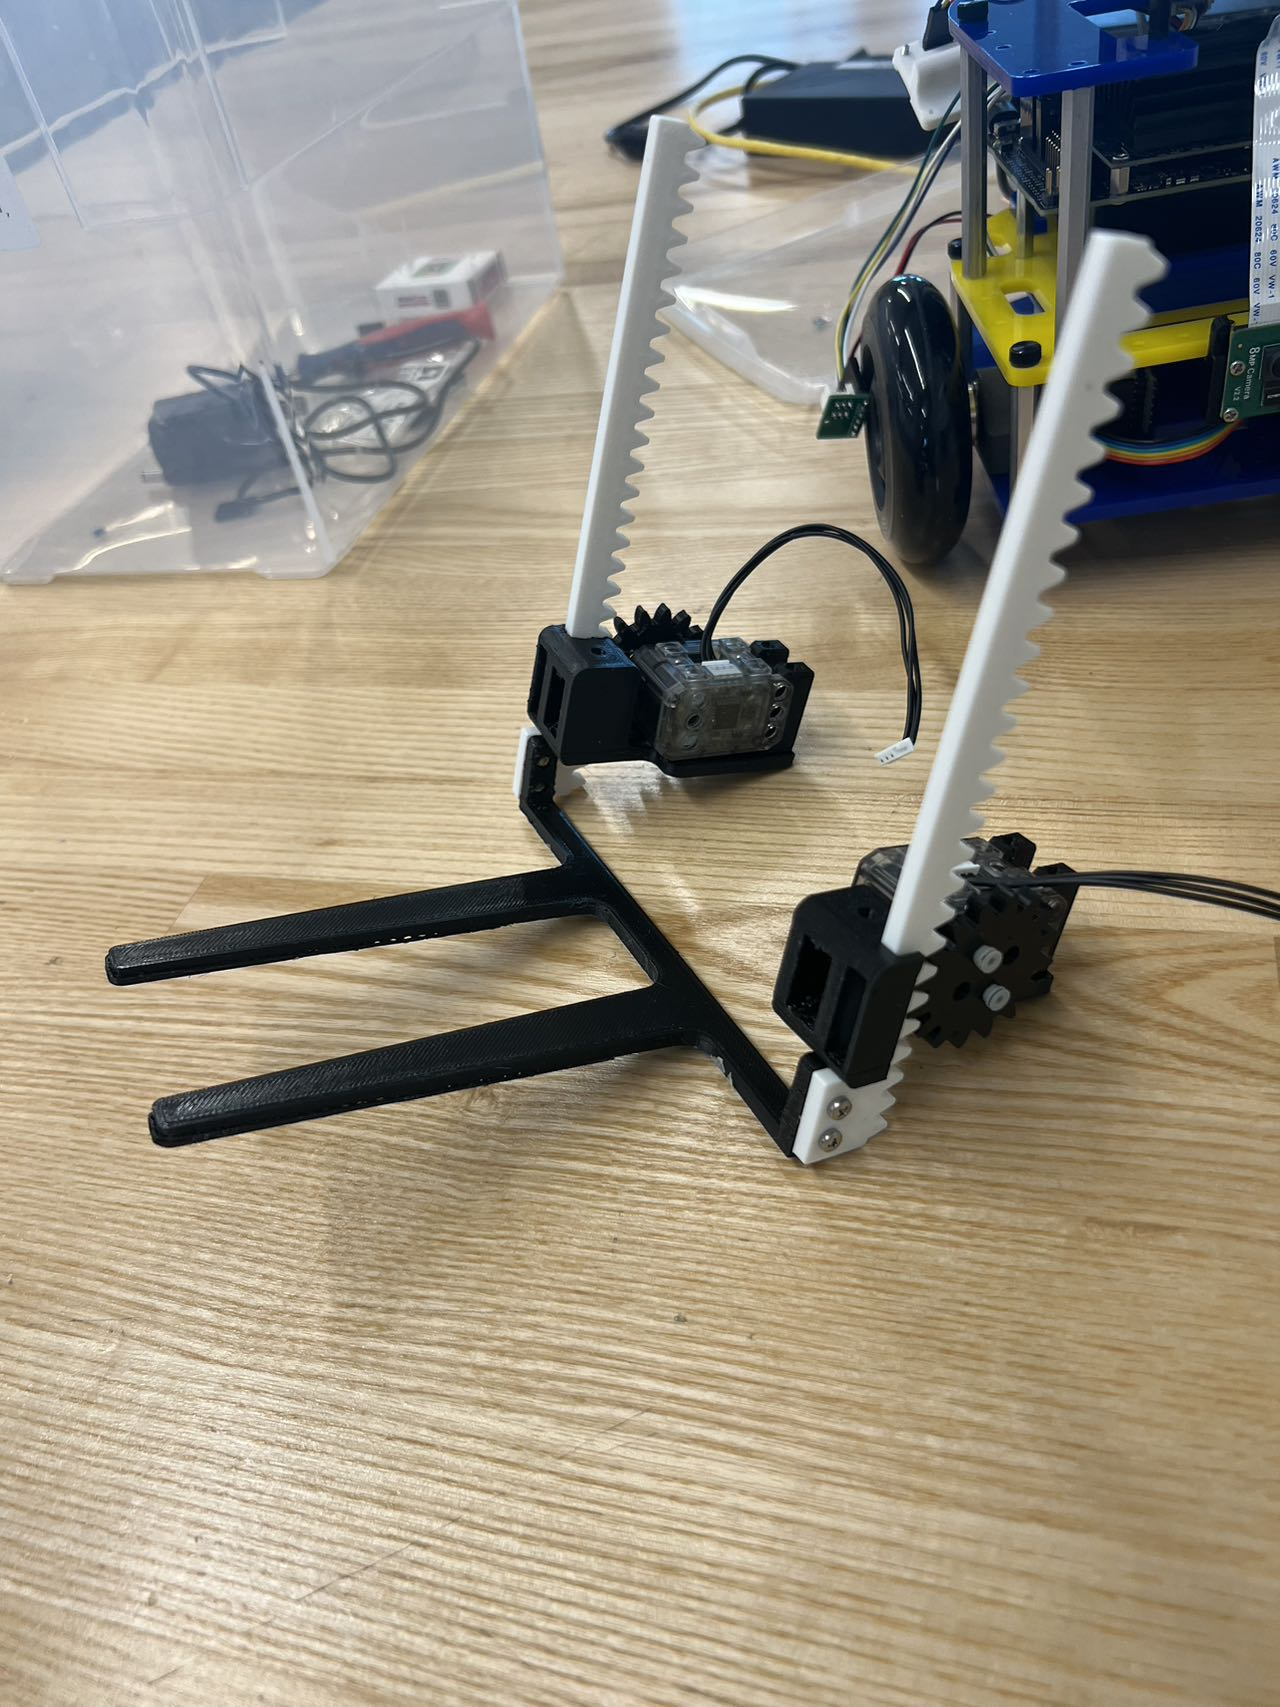
\includegraphics[width=\linewidth]{7.jpg} 
            \caption{}
        \end{minipage}
    \end{figure}

    \newpage
    

    \item \textbf{Link the forklift with the robot:}
    Link each gear box with robot by two 2.5mm screws.
    \begin{figure}[H]
        \centering
        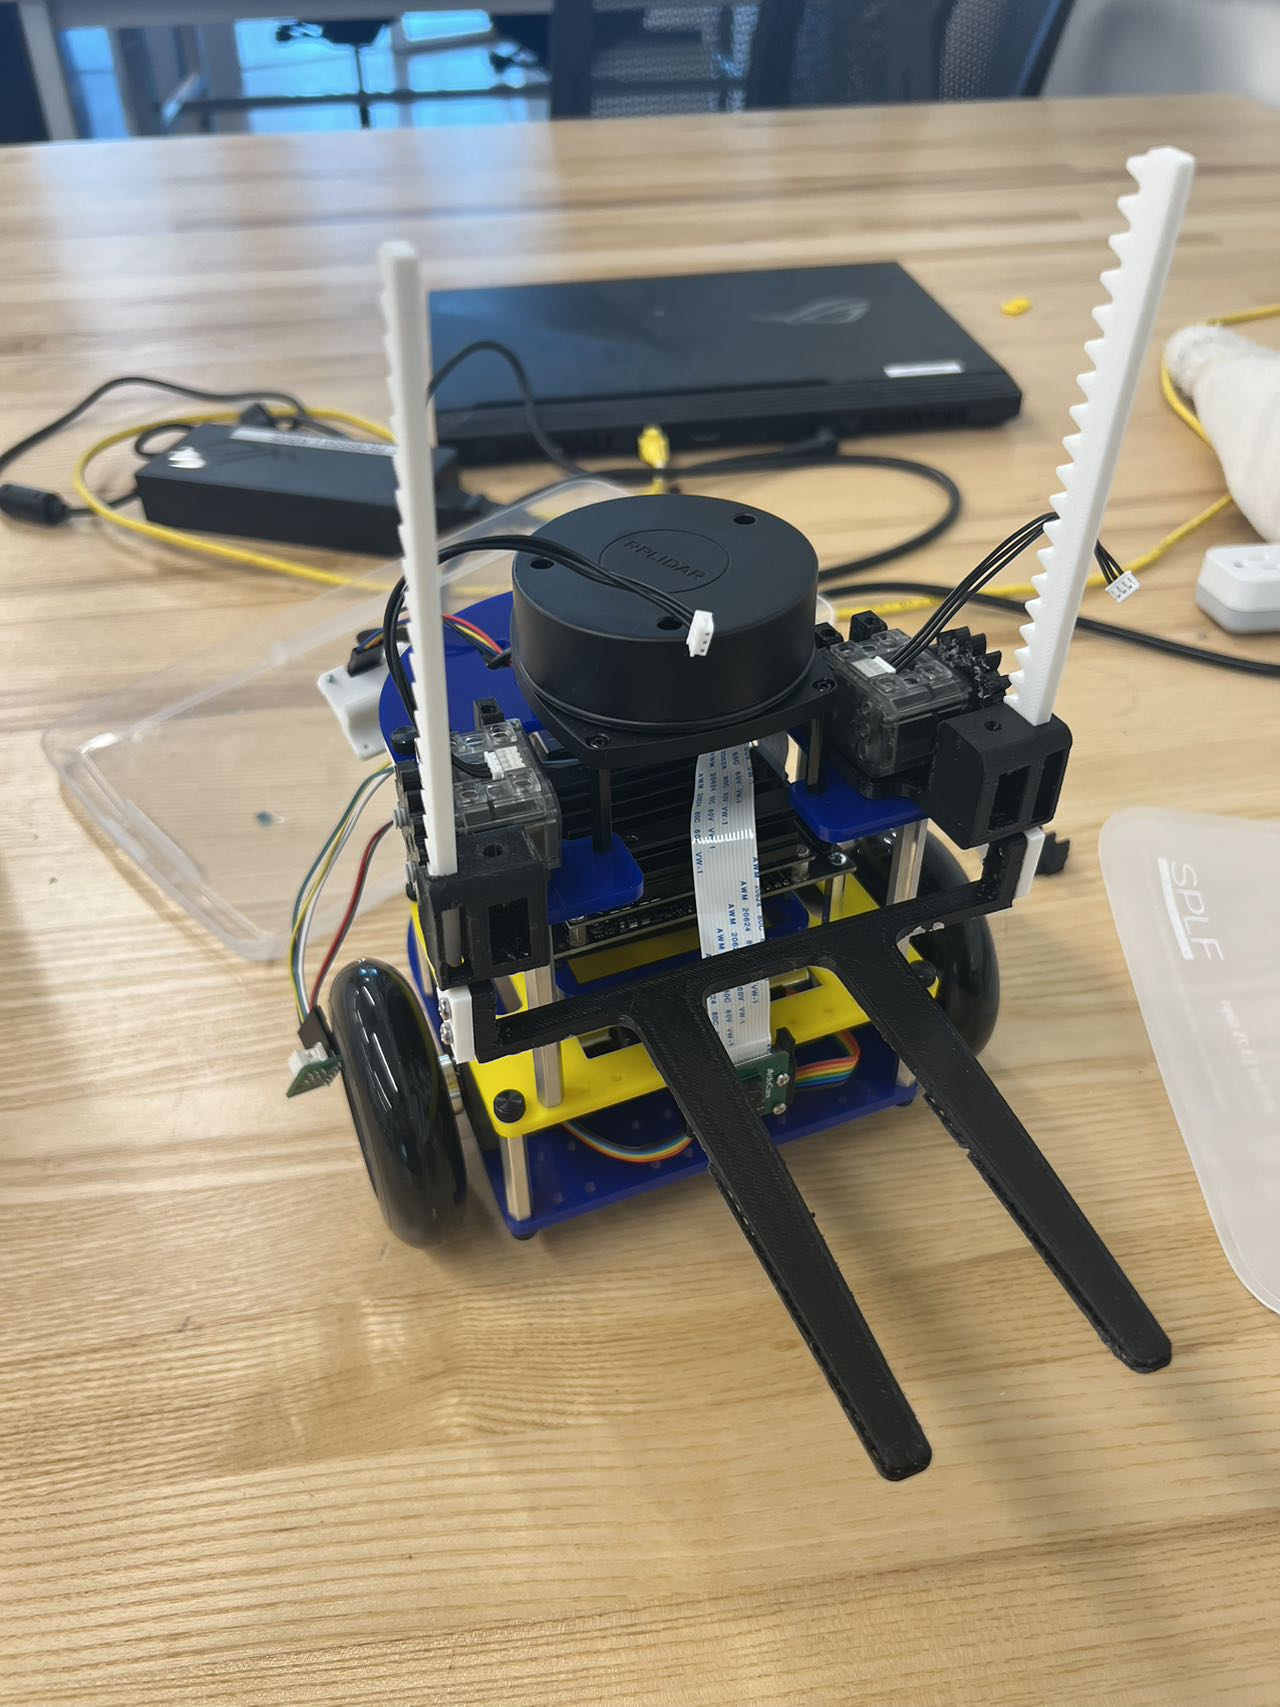
\includegraphics[width=0.40\textwidth]{8.jpg}
        \captionsetup{justification=centering}
        \caption{}
    \end{figure}  

    \item \textbf{Link signal cable with chip:}
    Link each signal cable with chip by two pins.
    \begin{figure}[H]
        \centering
        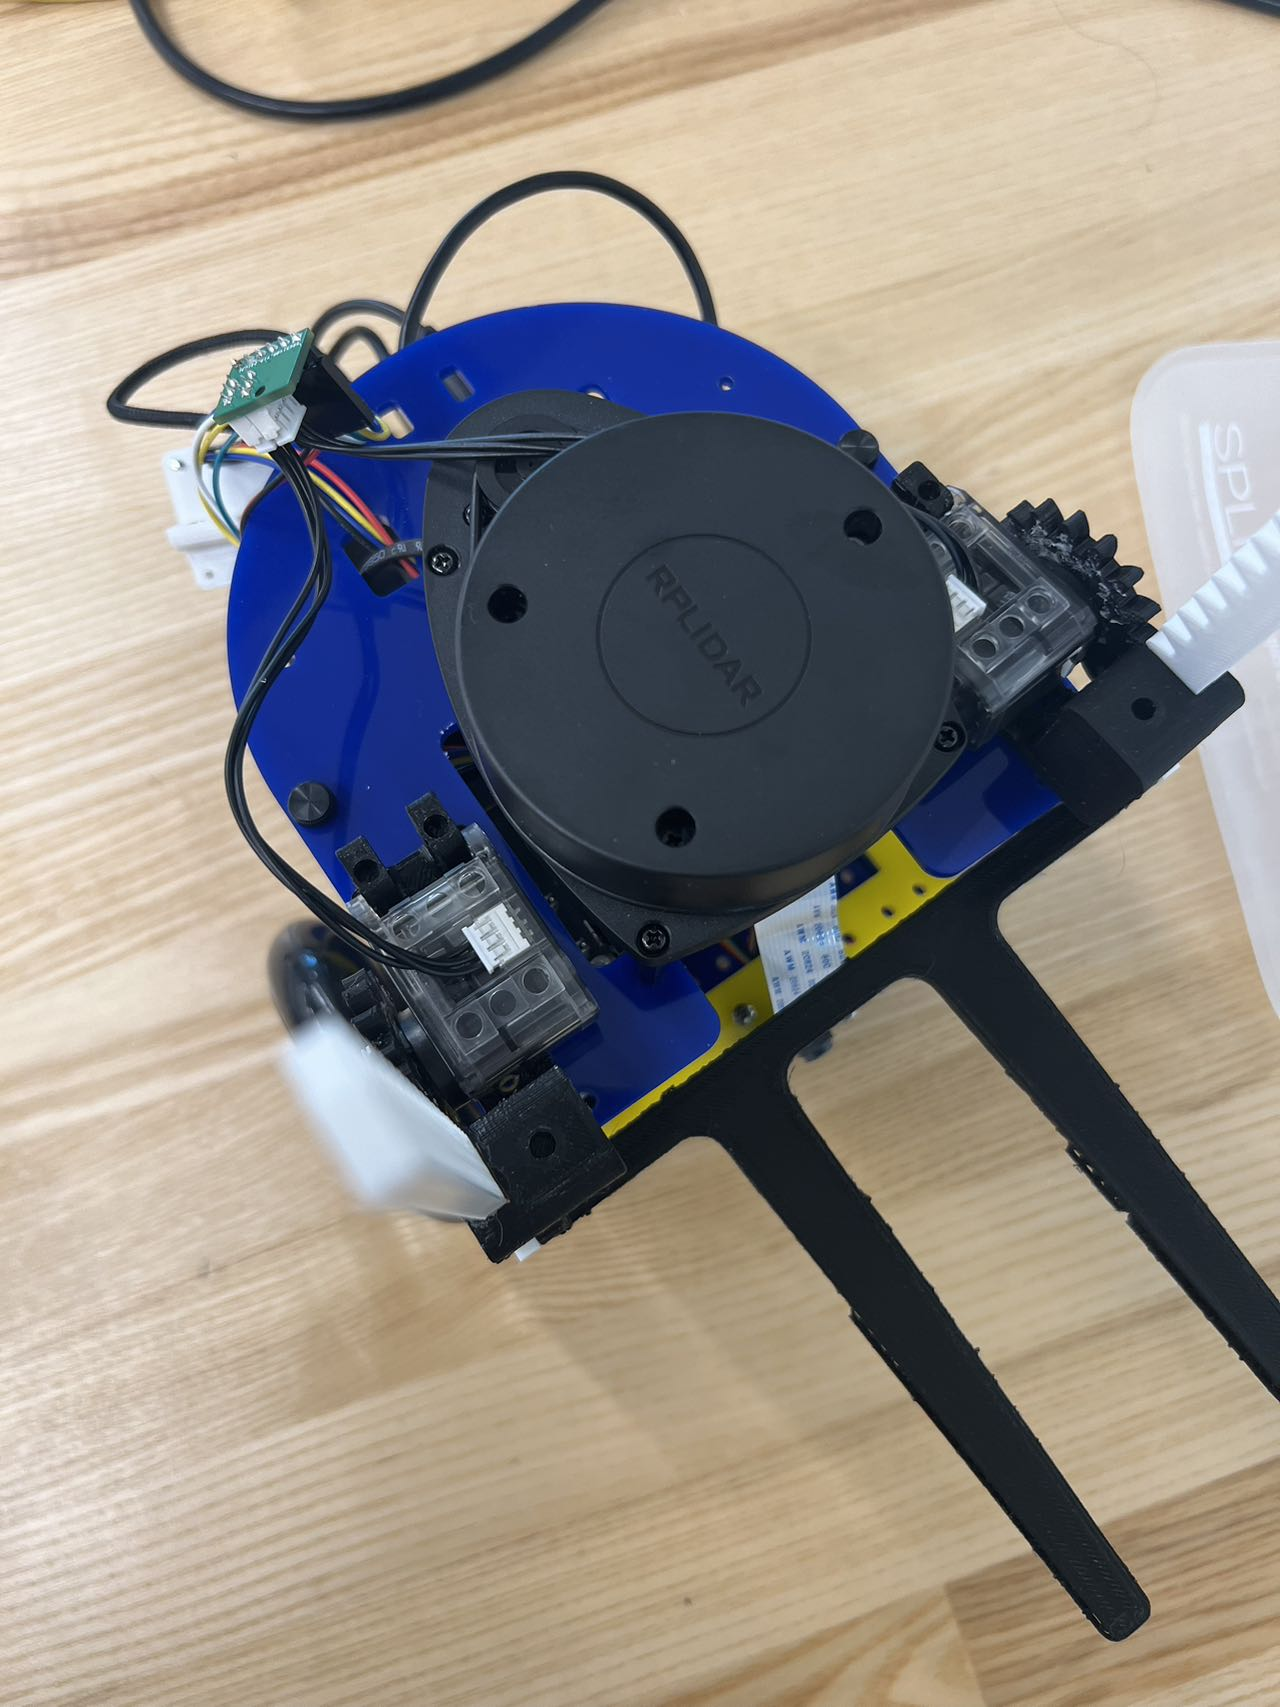
\includegraphics[width=0.40\textwidth]{9.jpg}
        \captionsetup{justification=centering}
        \caption{}
    \end{figure}  

   
\end{enumerate}

\section{Testing}
After assembly, test the forklift in various lifting conditions to ensure it operates correctly.

\end{document}